\section{Estática de los fluidos}

La \textbf{estática de fluidos} es el estudio de fluidos en los que no hay movimiento relativo entre sus partículas. Si no hay movimiento relativo, no existen gradientes de velocidad $\sfrac{du}{dy}$, por lo cual los esfuerzos cortantes serán nulos. El único esfuerzo que existe es un esfuerzo normal, la presión, de modo que ésta tiene la mayor importancia en este estudio.


\subsection{Presión en el seno de los fluidos}%Ver mejor este título

\subsubsection{Presión en un punto}

La presión en un punto de un fluido es constante, es decir, \textsl{la presión es una función escalar y no depende de la dirección normal del área}. Actúa igualmente en todas las direcciones.

\begin{equation}
	p_x = p_y = p_z = p
\end{equation}

%Esta imagen estaba por la demostracion pero me dio paja escribir todo, si quieren saquenla o dejenla, para que se entienda a qué van las p que están arriba...o sea, px py pz
\begin{figure}[H]
	\centering
	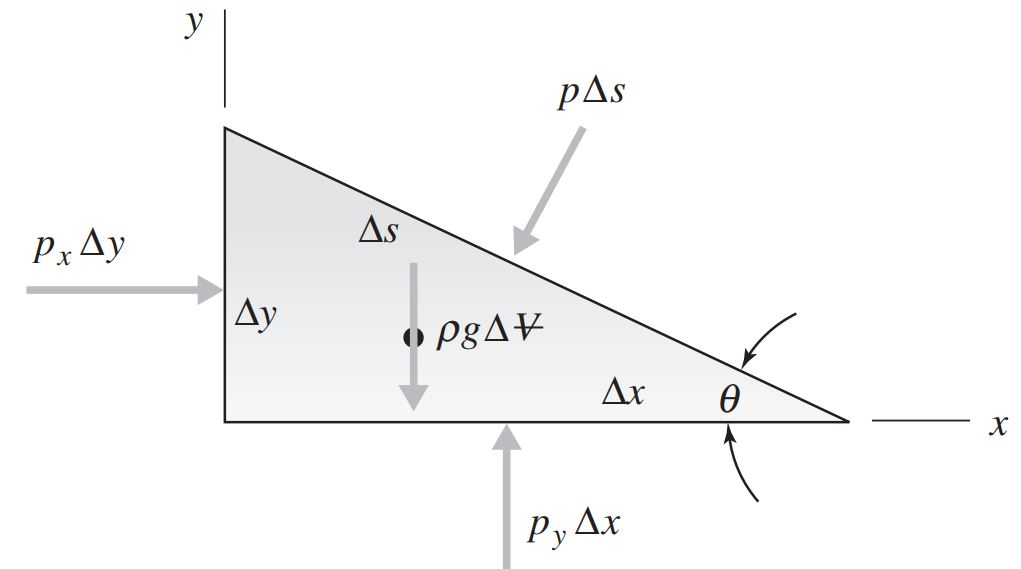
\includegraphics[width = .5 \linewidth]{fluido-infinitesimal}
	\caption{Presión en un punto en un fluido.}
	\label{fig:elemento-infinitesimal}
\end{figure}

\subsubsection{Variación de presión}

%Para determinar la variación de presión de fluidos en reposo, se considera el elemento infinitesimal que se ilustra en la figura \ref{fig:elem-infinitesimal}.
%
%\begin{figure}[H] 
%	\centering
%	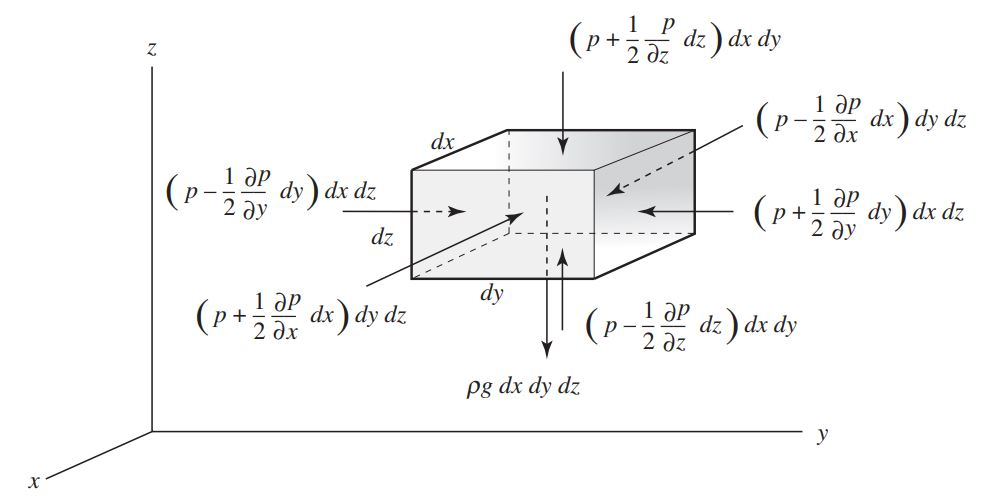
\includegraphics[width = .8\linewidth]{elemento-infinitesimal}
%	\caption{Fuerzas que actúan sobre un elemento infinitesimal de fluido.}
%	\label{fig:elem-infinitesimal}
%\end{figure}
%
%Las presiones en cada uno de los lados se pueden expresar utilizando la \textsl{regla de la cadena} del cálculo infinitesimal con $p\left(x,y,z\right)$:
%
%\begin{equation*}
%	dp = \dfrac{\partial p}{\partial x} dx + \dfrac{\partial p}{\partial y} dy + \dfrac{\partial p}{\partial z} dz
%\end{equation*}
%
%Si nos movemos una distancia $\dfrac{dx}{2}$, la presión será:
%
%\begin{equation*}
%	p\left(x + \dfrac{dx}{2},y,z\right) = p(x,y,z) + \dfrac{\partial p}{\partial x} \dfrac{dx}{2}
%\end{equation*}
%
%Considerando a la Ley de Newton en forma vectorial para un sistema de masa constante como la sumatoria de las fuerzas igualadas a la aceleración por su masa, se llega a tres ecuaciones de componentes:
%
%\begin{align*}
%	-\dfrac{\partial p}{\partial x}\ dx\ dy\ dz & = \rho a_x\ dx\ dy\ dz\\
%	-\dfrac{\partial p}{\partial y}\ dx\ dy\ dz & = \rho a_y\ dx\ dy\ dz\\
%	-\dfrac{\partial p}{\partial z}\ dx\ dy\ dz & = \rho (a_z+g)\ dx\ dy\ dz\\
%\end{align*}

Para determinar la variación de presión de fluidos se utiliza la ecuación \ref{eq:variacion-de-presion} que representa el diferencial de presión en cualquier dirección. 

\begin{equation}
	dp = -\rho a_x dx -\rho a_y dy -\rho (a_z + g) dz
	\label{eq:variacion-de-presion}
\end{equation}

En la estática de fluidos se trabajan con fluidos en reposo, es decir, que no tienen aceleración además de la que experimentan con la aceleración de la gravedad ($a_x = a_y = a_z = 0$).\\


Entonces, para dichos fluidos se llega a la \textbf{ecuación fundamental de la hidrostática}, donde la presión varía en la dirección vertical:

\begin{equation}
	\dfrac{dp}{dz}= - \gamma = - \rho\ g
	\label{eq:fundamental}
\end{equation}

Tambien, tenemos que tener en cuenta que $dp$ se incrementa cuando $dz$ disminuye; esto es, la presión \textbf{aumenta} cuando nos movemos \textbf{hacia abajo} y disminuye cuando es hacia arriba.\\

Si se integra la ecuación \ref{eq:fundamental} se llega a:

\begin{equation}
	P_1 - P_2 = \gamma (z_2 - z_1)
	\label{eq:fundamental-integrada}
\end{equation}\\


Supongamos ahora que se tiene un fluido contenido en un vaso de precipitado como se ilustra en la figura \ref{fig:precipitado}. 

\begin{figure}[H]
	\centering
	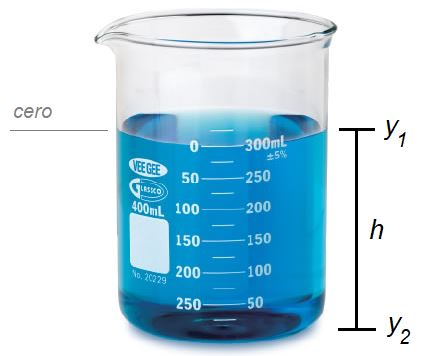
\includegraphics[width = .3\linewidth]{vaso-de-precipitado}\label{fig:precipitado}
	\caption{Presión en un fluido en reposo}
\end{figure}

Al estar en contacto con el aire, la presión en el punto 2 será la atmosférica $P_{atm}$, y la ecuación \ref{eq:fundamental-integrada} quedará de la siguiente manera:

%Falta...
\begin{tikzpicture}
	% Ejes cartesianos
	\draw[gray, thick] (0, 0) -- (4, 0) node[right] {$x$};
	\draw[gray, thick] (0,0) -- (0, 4.5) node[right] {$y$};
	
	% Estilo de la función lineal decreciente
	\tikzset{funcion/.style={black, thick}}
	
	% Función lineal decreciente
	\draw[funcion] (1.01325, 4) -- (1.01325+1, 0) node[right] {$P_1(h) = P_{atm} + \gamma\ h$};

	
\end{tikzpicture}



\begin{equation}
	P_1 - P_{atm} = \gamma (z_2 - z_1)
\end{equation}


A la diferencia $P_1 - P_{atm}$ se la denomina como \textbf{presión hidrostática}.\\



Si se despeja la presión $P_1$ se llega a la expresión para el \textbf{Segundo Principio de Pascal}:

\begin{equation}
	P_1 = P_{atm} + \gamma h
\end{equation}
\subsection{Ecuaciones fundamentales}

\subsection{Manómetros} %Ver este también

\subsection{Fuerzas sobre superficies}

\subsection{Cuerpos sumergidos}

\subsubsection{Empuje de flotación}

\subsubsection{Estabilidad de flotación}

\subsection{Equilibrio relativo}	
